\documentclass[
  journal=largetwo,
  %manuscript=review,
  year=2025,
  volume=37,
]{cup-journal}

\input{preamble.tex}
\input{math_commands.tex}

\addbibresource{references.bib}

\title{Learning theoretic reformulation and double descent}

\author{Bui Gia Khanh}
\affiliation{Department of Physics, Hanoi University of Science, Vietnam National University, Hanoi Vietnam}
\email[Bui Gia Khanh]{fujimiyaamane@outlook.com}

%\addbibresource{references.bib}

\keywords{Statistical learning theory, double descent, deep learning, computational complexity theory, complexity theory, grokking} %% First letter not capped

\begin{document}
\begin{abstract}
    The analysis of learning action, machine learning and related practices in the field theoretically has been made by utilizing Computational Learning Theory (CoLT) \cite{10.1145/1968.1972} and Statistical Learning Theory (SLT) \cite{Vapnik1999-VAPTNO}. These two theories, while overlapped, provides a general framework in analyzing and justifying learning actions and learning model constructions, aiding in the formation of modern practices. One of the famous insight using such framework is the \textit{bias-variance tradeoff} \cite{6797087}, which states that model complexity and generality inversely affect each other, thus guarantee the need for a safe bracket between them. However, recent literatures, \cite{belkin_reconciling_2019} has indicated the fallout of such dilemma by the new phenomenon called \textit{double descent}, where there exists an interpolation threshold that renders the current statistical justification for bias-variance inconsequential to a given region. Various `anomaly' has also been detected similarly, with varying degree of sophistication and potential.In this paper, we would like to review through progress made in this particular field of research, and the phenomena potential explanations up until now. 
\end{abstract}
\section{Introduction}
\begin{figure*}
  \centering
  
\includegraphics[width=0.7\textwidth]{g10.png}
  \caption{{\small \textbf{Illustrative dynamic of the learning problem.} For an incremental hypothesis space sequence $\mathcal{H}_{1},\mathcal{H}_{2},\mathcal{H}_{3}$, we aim to obtain the procedure $\mathcal{T}$ that would either reach the \textit{generalization solution} $\bm{h}$, or the \textit{empirical solution} $h^{*}$ for a particular hypothesis class, with respect to the concept $c$ and its observed concept $c'$. Model selection hence dictates how an algorithm or procedure than choose the best possible hypothesis to approximate the generalization solution from the empirical solution set. Do notice that here we explicitly state that the data would create a \textbf{proxy concept} that overlaps with the concept class and of some arbitrary `distance' from the true concept by $d(c,c')$. In case the two classes overlap, there still exists the arbitrary distance. Also, we can also observe the intuitive notion of increasing hypothesis class - while it indeed can help in getting closer to the concept class, the somewhat intrinsic property of current learning theory being the relative random procedure class make it probabilistically unstable.}}
  \label{fig:statlearnclassical}
\end{figure*}
The modern machine learning landscape is dominated and guaranteed by the foundation of theoretical machine learning, specifically computational learning theory (CoLT) and statistical learning theory (SLT). The theory of machine learning and its modern practice has been developed and researched, of a substantial portion by empirical and heuristic approach, either by advancing new practices, architectures or by try-and-test modification. From its early onset of a regression estimator $\theta(x,y)$ on the linear regression problem, machine learning has developed substantially. Certain model concept with great successes includes regression-classification model, Bayesian modelling, generative learning model, support vector machine, Gaussian processes, and more. Of all such, the more formal and complex model architecture created, is the concept of a \textit{neural network}. With increasingly sophisticated architecture, heuristic approach become popular, the fast-paced advancement of the field comes with new method, new results, new observations, and its far-reaching application which led to even bigger and larger scale deployment, there has been questions about the formation and status of a theoretical ground, a rigorous matter on the side of \textbf{theoretical machine learning}.

While rigorous and well-formulated in a sense, classical and theoretical machine learning was dwarfed by the modern advancement of machine learning as a whole, leading to several anecdotal problems regarding the interpretation of phenomena, the re-evaluation of the theory to fit the more updated analysis, and explanation to more sophisticatedly designed system. This and many more, plus as present, many of such advancements and improvements are heuristic, and the general theory and conceptual understanding remain limited, led to the choice to often opt for analogies and empirical workaround. Ultimately, this resulted in multiple `failures' in explaining, interpreting, and predicting behaviours of new phenomena appeared in the modern landscape of machine learning. While there exists novelty of analysis, and different theoretical schemes to analyze such, particular problems remain in the form of irregularity and conflict of interpretations between frameworks. 

The main focus is to review on the topic, analyse existing analysis and observations, and understanding of the umbrella term classical learning theory, for the recent phenomena observed named `double descent'. Statistical learning theory (SLT) and computational learning theory (CLT) \cite{Vapnik1999-VAPTNO,10.5555/2371238,10.5555/2621980,STL_Hajek_Maxim_2021,bousquet2020theoryuniversallearning} has been prominent in constructing a well-rounded formal theory surrounding learning problems, models, and machine learners analysis. Valuable insights have been dissected from treatment of statistical theory and mathematical modelling on models, including the \textit{bias-variance tradeoff} \cite{6797087,Domingos2000AUB}, which serves as a bound for efficient learning and model configuration (or complexity). However, recently there has been observations of \textit{double descent} \cite{belkin_reconciling_2019,schaeffer_double_2023,nakkiran_deep_2019,lafon_understanding_2024} which refute the famous tradeoff assumption, and hence brings question to the establishment of the theory, as well as several assumptions and insight in the framework. Further events and phenomena observed also includes grokking and triple, to $n$-descent \cite{davies_unifying_2023,d_ascoli_triple_2020}. Furthermore, many problems of defining and formalizing notions used in designing and implementing machine learning models are inconclusive, such as, for example, \textit{model complexity} and others. 


\section{Methodology and Experiments}

Since most of the progresses are in particular theoretical, our research focus on both \textbf{theoretical analysis} on the side of learning theory, statistical learning theory, and modern network landscapes; in addition to certain experimental results as for probing double descent on their grounds. In particular, we found out that you can inject dynamical \textbf{model control space} on $(m,|\mathcal{H}|)$-configuration hypothesis space, as seen in Hypothesis~\ref{hyp:interpolation_tau}.
\begin{hypothesis}[The flawed PAC-descent]\label{hyp:interpolation_tau}
    Let $\mathcal{H}$ be the hypothesis class, for moving parameter $\tau$ called the \textbf{interpolation threshold}. We define the interpolation offset region, $\Delta(\tau)\equiv\Delta := \tau-p$, and the regularized deviation term $\eta,\kappa>0$. Then, for specific $q(\tau)$, where we set $\tau=|\mathcal{H}|$ of the hypothesis class size, and $\tau=m$ case of the number of samples on $\mathcal{S}$, then $R(h_{\mathcal{S}})$ is bounded by, for at least probability of $1-\delta$: 
    \begin{equation}
        \begin{split}
            & R(h_{\mathcal{S}})\\
            &\leq \begin{cases}
            \frac{1}{m} \left( \log{|\mathcal{H}|} + \log{\frac{1}{\delta}} \right) & \Delta \leq -\gamma \\
            \frac{1}{m} \left( \log{|\mathcal{H}|} + \log{\frac{1}{\delta}} \right) + \lambda(\Delta) I \sqrt{\frac{log{(\tau - p)+\log{(2/\delta)}}}{2(\tau-p)^{\epsilon}+1}} & |\Delta <\gamma| \\
            \frac{1}{m} \left( \log{|\mathcal{H}|} + \log{\frac{1}{\delta}} \right) + I\sqrt{\frac{log{(\tau - p)+\log{(2/\delta)}}}{2(\tau-p)^{\epsilon}+1}} & |\Delta <\gamma| 
        \end{cases}
        \end{split}
    \end{equation}
    for $I>0$, $\lambda(\Delta)\in[0,1]$ the smooth terms on transition region, where taking $\gamma =0, \lambda(0)=1/2$ returns the discrete separation case. 
\end{hypothesis}
We also attempted to re-interpret and reformalise learning theory, as seen of the conjunctive optimization problem of both generalization and empirical learning and their more general notion, in Illustration~\ref{fig:statlearnclassical}. Because the problem is focused on double descent, theoretical effort and experiments mostly focused on such. As far as literature are considered, double descent remains a problem that is very hard to manifest, and often time require consistent and constrained experimental regime for it to be observable. Hence, our method is then to \textbf{stress-test} until we can find double descent in any particular model class. In particularly interesting case, for results and stress-testing on a specific linear-multilinear model under least-square analytical solver, double descent is predicted and conjectured to have irregular collapse and abnormal mismatch between different internal structure to external inference error risk objective class. 

\begin{figure}[htb]
    \centering
    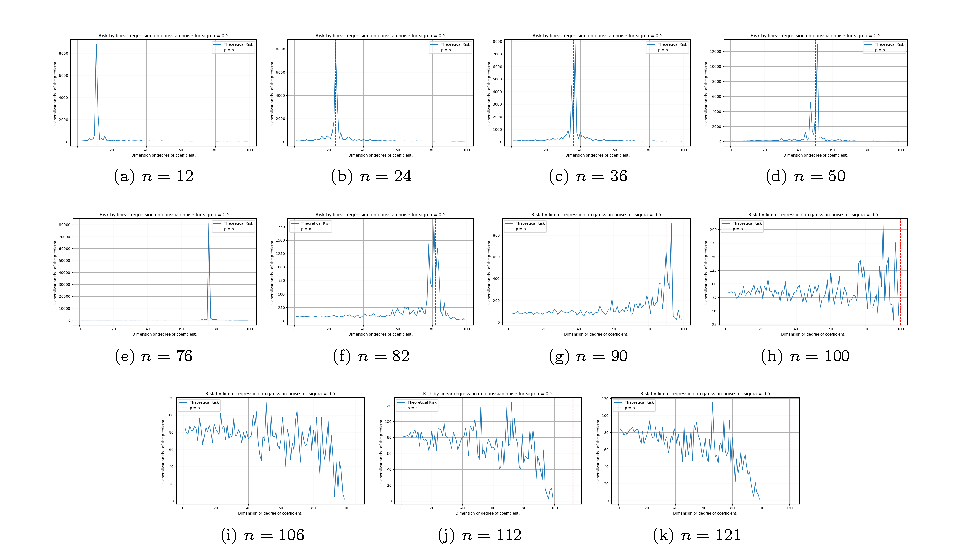
\includegraphics[width=\textwidth]{pdf/theorem_2.pdf}
    \caption{Contrary to theorem from \cite{lafon_understanding_2024}, this is the behaviours on randomized setting for standard parameter-wised mean square error measure (MSE-on-parameter). For this model, we have $d=100$, $\sigma = 0.5$, and variational $n$. Full test cases are for $p=[1,100]$, $n=\{12,24,36,50,76,82,90,100,106,112,121\}$ accordingly. The test function of the concept itself is the same linear model, but with different input only.}
    \label{fig:theorem_double_descent_fig2}
\end{figure}

Further experiments includes multi-polynomial models, neural networks under componential formalism, and Graph Neural Network (GNN) in particular specificity, and yielded various interesting results, but we deliberately do not include it in such state to this report because of length depth. The paper itself is in its final state, and should be able to be published once experiments are quantitatively analysed further during evaluation. 

\clearpage

\printbibliography



\end{document}